%\documentclass[twocolumn]{article}
\documentclass[11pt]{article}
\usepackage{indentfirst}
\usepackage{amsmath,amsthm,amssymb}
\usepackage{fancybox}
\usepackage{fancyvrb}
\usepackage{minted}
\usepackage{color}
\usepackage{makeidx}
\usepackage{xeCJK}
\setCJKmainfont[BoldFont={Adobe Heiti Std}, ItalicFont={AR PL New Kai}]{Adobe Song Std}
\usepackage{graphicx}
\usepackage{geometry}
\usepackage{amsmath}
\usepackage{amsfonts}
\usepackage{array}
%\usepackage{tikz}
\usepackage{gnuplot-lua-tikz}
\usepackage{cite}
\usepackage{url}
\geometry{left=1.5cm, right=1.5cm, top=1.5cm, bottom=1.5cm}
\usepackage{wrapfig}
%\usepackage{lettrine}
%\usepackage{abstract}

% THEOREMS -------------------------------------------------------
\newtheorem{Thm}{Theorem}
\newtheorem{Cor}[Thm]{Corollary}
\newtheorem{Lem}[Thm]{Lemma}
\newtheorem{Prop}[Thm]{Proposition}
\newtheorem{Prob}{Problem}
\theoremstyle{definition}
\newtheorem{Def}[Thm]{Definition}
\newtheorem*{Sol}{Solution}
\theoremstyle{remark}
\newtheorem{Rem}[Thm]{Remark}
\numberwithin{equation}{section}
% MATH -----------------------------------------------------------
\newcommand{\norm}[1]{\left\Vert#1\right\Vert}
\newcommand{\abs}[1]{\left\vert#1\right\vert}
\newcommand{\set}[1]{\left\{#1\right\}}
\newcommand{\Real}{\mathbb R}
\newcommand{\eps}{\varepsilon}
\newcommand{\To}{\longrightarrow}
\newcommand{\BX}{\mathbf{B}(X)}
\newcommand{\A}{\mathcal{A}}
\newcommand{\CommentS}[1]{}
% CODE ----------------------------------------------------------
\newenvironment{code}%
{\vglue 5pt \VerbatimEnvironment\begin{Sbox}\begin{minipage}{0.9\textwidth}\begin{small}\begin{Verbatim}}%
{\end{Verbatim}\end{small}\end{minipage}\end{Sbox}\setlength{\shadowsize}{2pt}\shadowbox{\TheSbox}\vglue 5pt}


\usepackage{pgf}
%\usetikzlibrary{arrows,automata}
%\usepackage[latin1]{inputenc}
\usepackage{verbatim}
\usepackage{listings}
%\usepackage{algorithmic} %old version; we can use algorithmicx instead
\usepackage{algorithm}
\usepackage[noend]{algpseudocode} %for pseudo code, include algorithmicsx automatically

\lstdefinelanguage{Smalltalk}{
  morekeywords={self,super,true,false,nil,thisContext}, % This is overkill
  morestring=[d]',
  morecomment=[s]{"}{"},
  alsoletter={\#:},
  escapechar={!},
  literate=
    {BANG}{!}1
    {UNDERSCORE}{\_}1
    {\\st}{Smalltalk}9 % convenience -- in case \st occurs in code
    % {'}{{\textquotesingle}}1 % replaced by upquote=true in \lstset
    {_}{{$\leftarrow$}}1
    {>>>}{{\sep}}1
    {^}{{$\uparrow$}}1
    {~}{{$\sim$}}1
    {-}{{\sf -\hspace{-0.13em}-}}1  % the goal is to make - the same width as +
    %{+}{\raisebox{0.08ex}{+}}1		% and to raise + off the baseline to match -
    {-->}{{\quad$\longrightarrow$\quad}}3
	, % Don't forget the comma at the end!
  tabsize=2
}[keywords,comments,strings]

\lstloadlanguages{C++, Lisp, Haskell, Python, Smalltalk, Mathematica, Java}

\makeatletter
\newcommand\ackname{Acknowledgements}
\if@titlepage
  \newenvironment{acknowledgements}{%
      \titlepage
      \null\vfil
      \@beginparpenalty\@lowpenalty
      \begin{center}%
        \bfseries \ackname
        \@endparpenalty\@M
      \end{center}}%
     {\par\vfil\null\endtitlepage}
\else
  \newenvironment{acknowledgements}{%
      \if@twocolumn
        \section*{\abstractname}%
      \else
        \small
        \begin{center}%
          {\bfseries \ackname\vspace{-.5em}\vspace{\z@}}%
        \end{center}%
        \quotation
      \fi}
      {\if@twocolumn\else\endquotation\fi}
\fi
\makeatother
%--------------Now the document begins------------------

\author{Jingcheng Liu ~(~刘景铖~) \thanks{F1003028(ACM Honored Class) 5100309243 \texttt{Liuexp@gmail.com} ~ } }

\title{Design and Implementation of SJTU-Schemer \\ \large a Purely Functional Approach}
\begin{document}
\maketitle

\section{Introduction}
\subsection{Usage}
要使用命令行下面的解释器,请在schemer根目录下面执行make.
test.scm中包含了一些可供测试用的代码.

要使用在线版解释器,请在schemer/web目录下面执行\verb|cabal install|.
接下来请在相同目录下面执行\verb|web -p 8000|.
之后可以访问\url{http://localhost:8000/parser/}和\url{http://localhost:8000/schemer/}查看不同实现效果.
\subsection{Screenshot}
  \begin{center}
    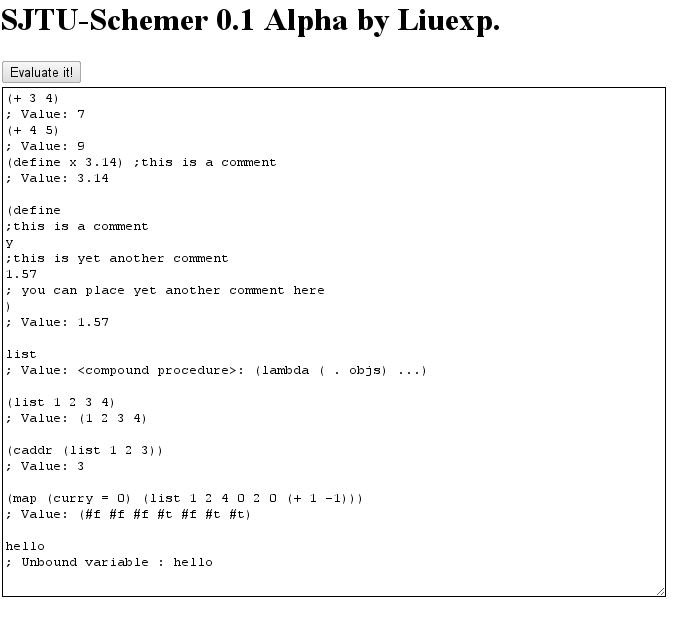
\includegraphics[width=0.40\textwidth]{a.png}
    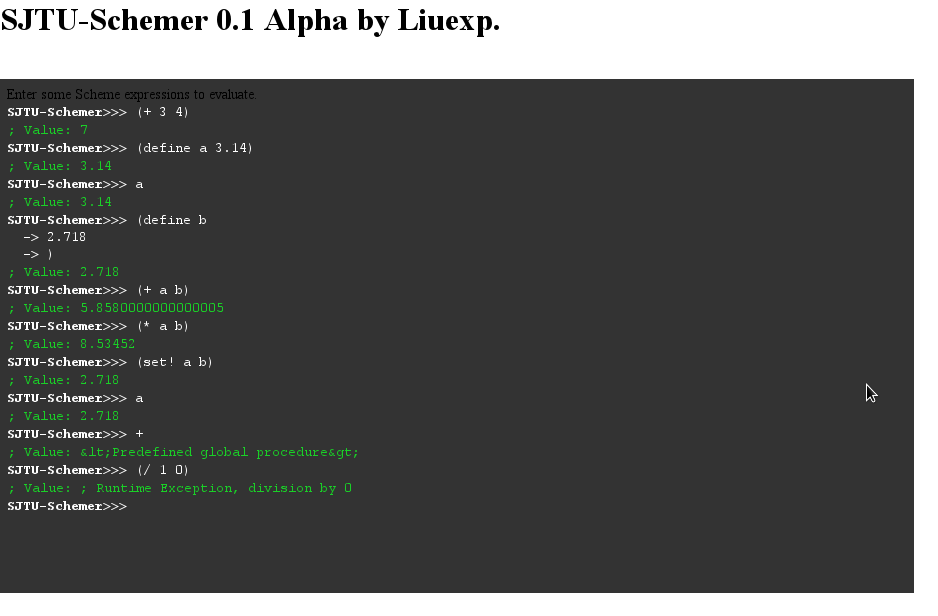
\includegraphics[width=0.53\textwidth]{b.png}
  \end{center}
\begin{center}
    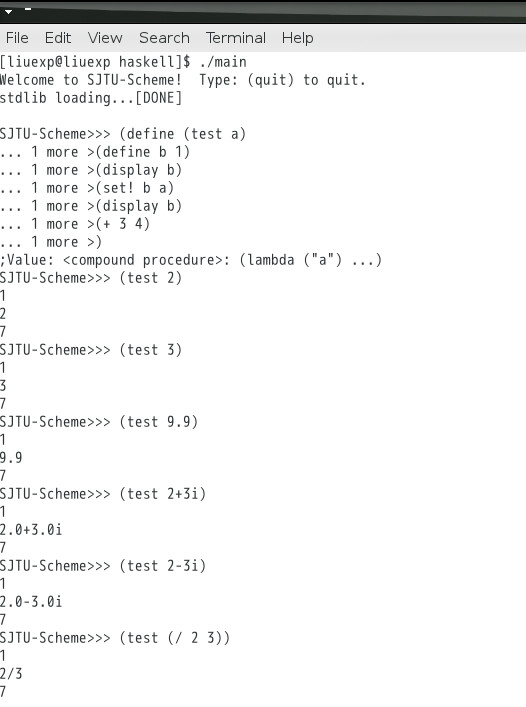
\includegraphics[width=0.40\textwidth]{c.jpg}
    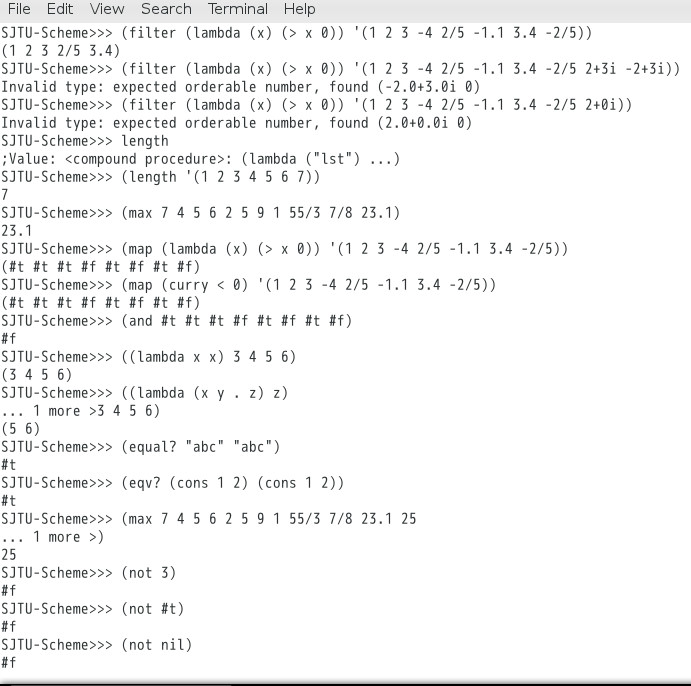
\includegraphics[width=0.53\textwidth]{d.jpg}
  \end{center}
\begin{center}
    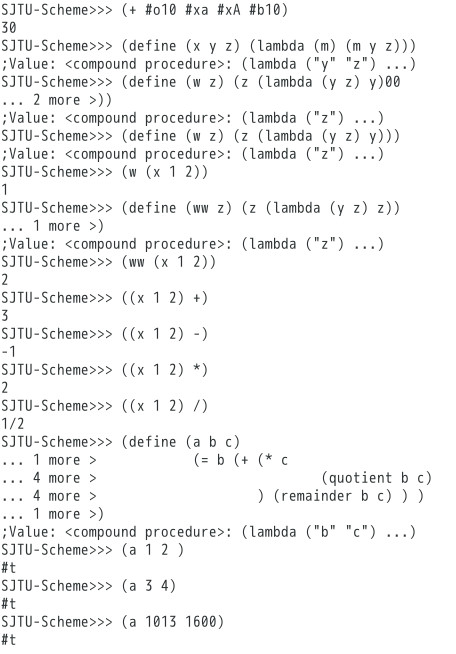
\includegraphics[width=0.40\textwidth]{f.jpg}
    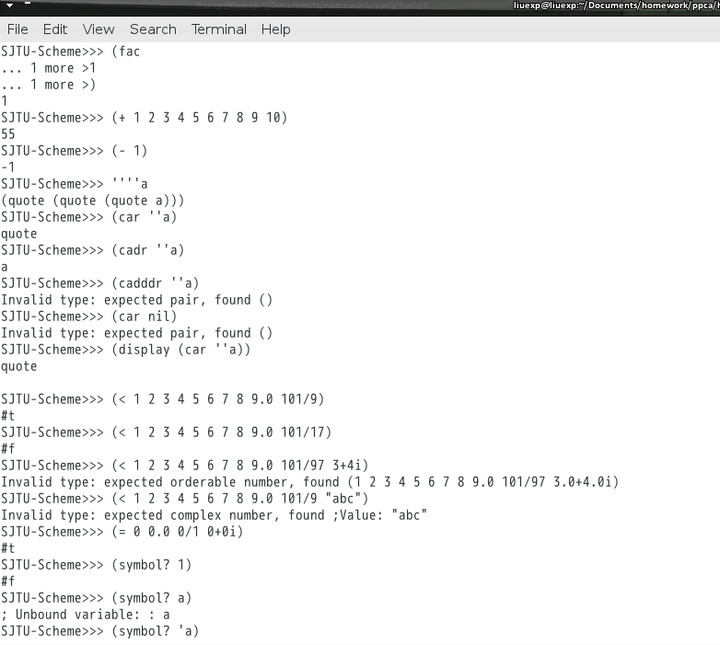
\includegraphics[width=0.53\textwidth]{e.jpg}
  \end{center}

\section{Basic Framework}
\subsection{Monad}
由于本文介绍的解释器是基于Haskell语言实现的,
这里简单介绍一下里面的Monad.

首先,对于纯函数式代码来说,一切行为是完全确定的,
也就无法直接和现实世界交互,因为现实世界的行为
和参数都是不确定的。这就需要一些介质来与现实世界
交互了,Haskell里面就是通过Monad来实现的,也就是
通过Monad来把纯函数式代码与那些将直接与现实世界
交互的代码分离开来。

Monad的出现主要是为了简化一些计算步骤的组合过程的.
就像Java中的try..catch..finally一样,不过不同的是
Monad要比它更简洁,不同的Monad实际上是对计算过程的不同组合方式.

比如说Maybe Monad是用于那些可能成功(则返回结果),也可能
失败(则什么也不返回)的过程的组合,就像命令式语言中我们
会返回0,-1,INT\_MAX一样,不过这些值本身是没有意义的,
Maybe Monad里面则有了明确意义.而MonadPlus在Maybe Monad下面的
组合将表现为如果有一个Maybe Monad里面成功了则返回里面的值,
否则什么也不返回(注意这也是在一个新的Maybe Monad下面).
这些过程都很常见,把它们的过程特征抽象成Monad只是极大的简化
了代码.

而有趣的事情是,这些计算过程什么时候能抽象成Monad,是需要
满足一些条件的,这些条件和范畴论中的Monad所要满足的条件是
完全一样的,这也是Haskell中会出现范畴论中的词语的原因.
\subsection{Parsing}
Scheme的语法结构比较简单,可以分两种,一种在
Lisp中被称为原子({\bf Atom}),意即不可再分的东西,
如一般的数字,字符串,符号,布尔值都属于原子;
另一种则是表达式,表达式用括号括起来.
另外空格是作为分隔符.

总的来说Parser还是比较好写的,不过也比较容易在一
些细节上面出现Bug,比如表达式前面的空格,
括号前后的空格等.

在引入注释之前可以直接把换行符全部替换成空格,
这样就可以处理多行的问题了.引入注释后就不能这么处理了,
一种方法是先处理掉注释,不过这里采用的方法是
在Parser中同步处理注释.

编写Parser时,一种方法是自己写,主要是实现两个过程,
一个是peek即向前看的,一个是eat就是处理掉一个字符的.
不过自己编写时如果没有做好模块化的话,后面修改起来
会非常困难,而且因为抽象层次不高,即使有Bug也只能在
测试中发现.另一种方法是直接使用已有的工具生成,如C++的
可以用Yacc,Java的可以用JavaCC,这些工具可以直接通过
BNF文法生成需要的Parser. 还有一种方法是使用一种既可以像
BNF文法那样编写Parser,还有一些现成的Parser来自由组合的
parser combinator library,如Haskell中的Parsec,Java中的
JParsec等.这里用的是Haskell中的Parsec.

下面是一段利用Parsec来处理list一类的表达式的示例,
它是在Parser这一Monad中进行的,返回值是Scheme Primitives类型.
其中\verb|char '('|即指让Parser吃掉这个字符.
而\verb|try ...|是指让Parser向前看看是不是有这么一些字符.
\begin{minted}[mathescape,linenos,numbersep=5pt,frame=lines,framesep=2mm]{haskell}
listParser :: Parser Primitives
listParser = do
	char '('
	try (skipMany space)
	x <- sepEndBy exprParser spaces 
	try (skipMany space)
	char ')'
	return $List $ filter (not . isComment) x
  \end{minted}
  下面一段则是处理复数类“原子”的一个Parser.
  这些过程中会有很多细节,比如复数并不总是$1+2i$,
  可能是$1-2i,-1+2i$之类的.而在显示的时候,如果虚
  部是负数那么就不需要加符号直接显示,如果是正数或0
  则需要加一个“+”后再显示等.

\begin{minted}[mathescape,linenos,numbersep=5pt,frame=lines,framesep=2mm]{haskell}
complexParser :: Parser Primitives
complexParser = do x <- (try realParser <|> numberParser)
		   z <- try (char '+') <|> char '-'
                   y <- (try realParser <|> numberParser)
                   char 'i' 
		   return $ Complex ( toReal x  :+ case z of
							       '+' -> toReal y
							       '-' -> (0 -). toReal $y
							       )

  \end{minted}
\subsection{Evaluation}
这一部分对于使用Python的同学可能会比较容易实现,
因为Python本来就有一个eval的函数.
用Python写的Scheme解释器如pyscheme等都采用了内置
的eval函数.

如果按照纯函数式代码与需要与外界交互的代码分离的
原则,那么这里的eval是应该属于纯函数式代码的.
不过仔细一想却发现并不是如此的,首先Scheme本身
并不是一门纯函数式编程语言,所以eval里面会涉及
赋值等改变环境,以及类似\verb|(display "sth")|这样
的直接的IO操作.

看起来把display当成直接返回会是一个解决方法,不
过这却是错误的,因为对于多条语句同时执行的过程中,
eval只能返回最后一条的执行结果,如果display正好处
于中间那就被跳过了.

所以无论如何,对于Scheme解释器,eval都是需要放进IO Monad的.
所以这里对于环境选择的也是IORef而不是STRef.

另外在Haskell 中引入完整的数值系统时可能会遇到一些麻烦.
因为在像Haskell这么强的类型系统中,要想像C++,Java,Python中那么随便地进行通用型数值运算是不可能的,每个过程都必须有其确定的行为,如取模接受的只能是整数,大于号是不接受复数的等等,在这种情况下面,要想给环境bind上一个通用的+,-,取模等运算符是不可能的(因为参数和返回值的类型不一致),相对来说,比较诱人的但是却是错误的做法则是在运算(eval)的过程中把+,-等也作为一种Special Form,因为这时能拿到运算时的参数列表,可以通过参数的类型来确定+,-等所需要的实例的计算过程了。
不过这样+,-就不能作为一个计算过程进行传递的了。我最后想到的比较简单的方法是环境中绑定的并不是真的+,-计算过程,而只是一个虚的接口,这样在这个虚的接口里面也只用在运算前先对参数作一个类型检查,然后就可以通过类型来确定+,-所需要的实例的计算过程了。
\subsection{Apply}
这一部分对于使用Python的同学可能会比较容易实现,
因为Python本来就有一个apply的函数.
用Python写的Scheme解释器如pyscheme等都采用了内置
的apply函数.

Eval和Apply的时候主要需要注意closure的问题.
下面用一个例子说明这里采用的解决方法.
\subsection{Closure}
不妨来看下面的代码.
\begin{minted}[mathescape,linenos,numbersep=5pt,frame=lines,framesep=2mm]{scheme}
(define (test x)
       (define y 1)
       (display y)
       (set! y x)
       (set! pi x)
       (display y)
 )
\end{minted}
 那么在全局中会绑定test这个symbol到一个procedure上面.
 不过procedure会比较特别一点,因为需要一个closure的东西
 来确保在内部可以访问并修改外部,但在内部新定义的东西
 却又不会影响外部. 所以在绑定到procedure的同时还会把定义
 这个procedure所在环境的引用绑定上去.
 当调用它,如执行\verb|(test 9)|时,就要在全局这个环境中找到test
 对应的这个过程,然后执行它,执行的时候会为test找到
 所在的closure,然后在里面给x绑定上9,\verb|(define y 1)|时就在这个
 独立于全局的closure中给y一个值,\verb|(set! y x)|并修改它为9,
 最后结束后全局的环境中y还是未定义的,但pi的值会被修改为9.
 \subsection{Continuation}
 Continuation可以直接借助Haskell的Cont Monad(Control.Monad.Cont)来实现。里面有callCC等函数.

\section{Online Interpreter}
在做好一个在命令行下面的后,可以开始想怎么做一个在线的,在线的本身并不是重点,重点在于如果有了一个在线的模型后,就有了一个通用的API接口可以让它用于其它用途,如手机等各种嵌入式的本质上也只是把运行的平台换一换罢了,接口基本上不需要什么变化。

不过如果是在Haskell下面的话,这种担心是多余的,Haskell语言设计中的机制——把纯函数式代码与需要和外界交互的代码分离,其中后者是被包装到了Monad中——这是借用自范畴论的思想,这也使得最后转换为在线版的过程非常的顺利——仅仅是加了一个Monad Transformer——把原来的IO Monad中的action就转换到了Snap.Extension Monad中了(一个Web服务器框架),原来的代码甚至不用作任何修改。当然,这并不是真的不用修改,在线版与本地命令行的很重要的区别是Web的安全问题,尤其像这样的解释器,如果直接基于源代码进行过滤毕竟是有安全隐患的,所以我采用的是直接把对应的如打开文件,修改文件等命令去掉。这个API接口倒是通用的了。

另外在线的解释器需要考虑的一个问题是,如何保存用户之前的环境.
在本地中我们可以采用curry的方式,在REPL的过程中一直调用这个
partially applied function来实现使用的一直是同一个环境.(这一行
代码太长故只保留了最核心的Monad Binding)
\begin{minted}[mathescape,linenos,numbersep=5pt,frame=lines,framesep=2mm]{haskell}
primitiveBindings >>= evalAndPrint 
\end{minted}

但在Web下面就不可以了,因为也没有REPL这个循环,用户
也不是单一的.
最简单的方法自然就是把代码保存下来.这也是这里采用的方法.

理论上是可以通过类似Http Session的方法来解决的,
又或者是通过数据库(但数据库如何保存一个procedure我
还没想到简单一点的解决方法,haskell中的数据库似乎也
只有那些一般SQL数据库中的原始的数据类型)

考虑我对这方面了解不多,所以这里实现了的
主要还是两方面的内容,一是类似MIT-Scheme通过edwin
嵌入到emacs编辑器的,通过一个编辑窗口,允许用户
在编辑的过程中,随时evaluate。另一个是受到tryhaskell的
启发,模仿本地的界面做出来的一个在线解释器.


\section{Further Reference}
\begin{itemize}
\item Java的可以参考Jscheme.
\item Python的可以参考pyscheme.
\item Haskell的可以参考Write Yourself a Scheme in 48 Hours.
\end{itemize}

\end{document}
